% A TikZ node's `align=` lines are `\halign` cells (tikz.code.tex:4256 `\unhbox\tikz@align@line@box\unskip\cr`); since
% 59y `\unhbox` puts the line's items into the cell, so its first item is the cell's first. A phantom there is the
% line's content (pdflatex: only that line is indented); LaTeXML's cell peel took it for padding, which a column takes
% at its widest cell's, shifting every line (2605.03603, IEEE_ACCESS/main.tex:954; A/B of 59y). Guard
% box_primitives::tikz_align_line_padding.
% oracle:  pdflatex 0 errors: c1 "Alpha" / "  Beta" (Beta after the phantom's width); c2 the same with a math phantom;
%   c3 the same with a space after the phantom; c4 "Optimal" / "   layered" (three control spaces before "layered")
% rows:    c1-c3 GREEN 59y (the phantom ends the peel as content: both lines at x=0, the phantom kept; c1's picture
%            width 52.08 is pdflatex's, c2/c3's 54.73/59.34 are Rust's — pdflatex 58.07/62.69 from `$v_1:$`'s width;
%            heights are Rust's in every row: 30.98 for pdflatex's 25.61pt)
%          c4 RED (control spaces are glue in TeX, the line's content; LaTeXML's padding model takes a cell's leading
%            space as padding, applied per column at its widest cell's — both lines move 20.76pt; Perl-origin,
%            Alignment.pm:567-568, 659; per-cell padding needs a ruling; witnesses 2605.02838 `{\large \qquad 1}`,
%            2605.14035)
% status:  GREEN rows asserted; RED row waits for the padding ruling
\documentclass{article}
\usepackage{tikz}
\begin{document}
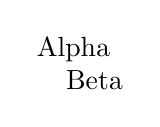
\begin{tikzpicture}\node[align=left] {Alpha\\\phantom{xx}Beta};\end{tikzpicture}

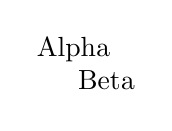
\begin{tikzpicture}\node[align=left] {Alpha\\\phantom{$v_1:$}Beta};\end{tikzpicture}

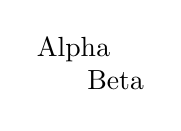
\begin{tikzpicture}\node[align=left] {Alpha\\\phantom{$v_1:$} Beta};\end{tikzpicture}

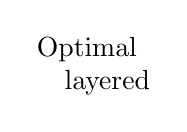
\begin{tikzpicture}\node[align=left] {Optimal\\ \ \ \ layered};\end{tikzpicture}
\end{document}
